\documentclass[aspectratio=169,8pt]{beamer}
\setbeamercolor{frametitle}{fg=black,bg=white}
\setbeamertemplate{frametitle}
{\begin{centering}\smallskip
    \insertframetitle\par
    \smallskip\end{centering}}
\setbeamertemplate{itemize item}{$\bullet$}
\setbeamertemplate{navigation symbols}{}

\setbeamertemplate{navigation symbols}{}
\setbeamertemplate{caption}{\raggedright\insertcaption\par}

\newcommand{\topline}{%
  \begin{tikzpicture}[remember picture,overlay]
   \node[xshift=0.5\paperwidth,yshift=-1cm] at (current page.north west){%
    
\includegraphics[width=\paperwidth]{i/line.png}};
  \end{tikzpicture}
}

\long\def\bframe#1#2\eframe{\begin{frame}{#1}\topline#2\end{frame}}
\long\def\bbframe#1\eframe{\begin{frame}#1\end{frame}}
\long\def\be#1\ee{\begin{align*}#1\end{align*}}
\long\def\bcc#1\ecc{\begin{columns}#1\end{columns}}
\long\def\bc#1\ec{\begin{column}{0.48\textwidth}#1\end{column}}
\newcommand{\fig}[1]{%
  \begin{center}
    \includegraphics[width=\textwidth]{#1}
\end{center}}
\newcommand{\wfig}[2]{%
  \begin{center}
    \includegraphics[width=#1\textwidth]{#2}
  \end{center}}
\newcommand{\ffig}[2]{%
    \includegraphics[width=#1\textwidth]{#2}}

\usepackage{tikz}
\usepackage{helvet}
%\usepackage[export]{adjustbox}
%\usepackage{makecell}


%\pdfpageheight=1920pt
%\pdfpagewidth=1080pt

\begin{document}

\bframe{RL for Fuid Mechanics}
aphros: flows with surface tension and chemical kinetics (Petr)
\newline
Nek5000: spectral element method, FORTRAN 77 (Jane, Martin, )
\newline
LAMMPS: particles (Ivica, Lucas, Pantelis, Pascal)
\newline
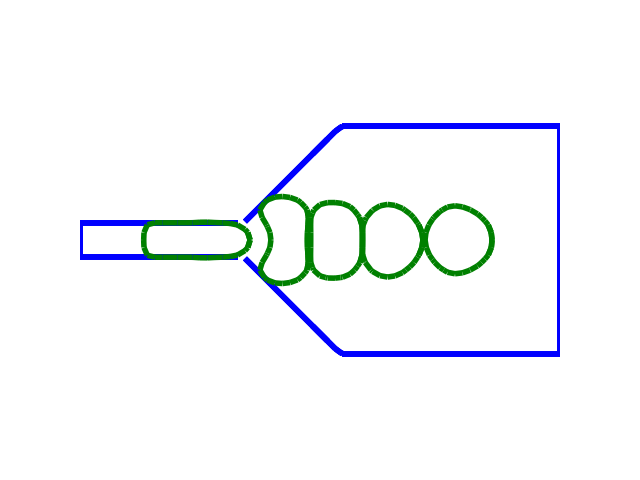
\includegraphics[width=0.29\textwidth]{i/aphros.png}
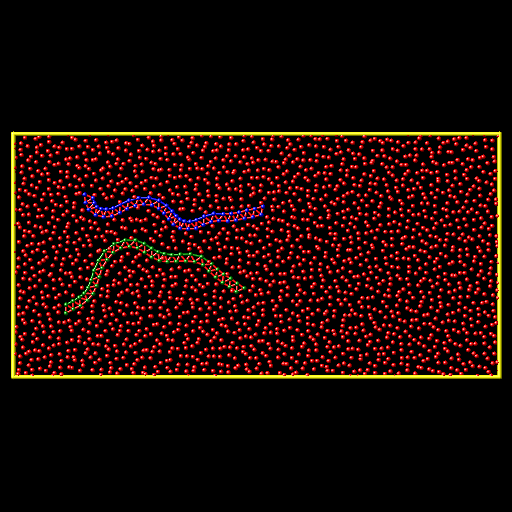
\includegraphics[width=0.29\textwidth]{i/lammps.png}
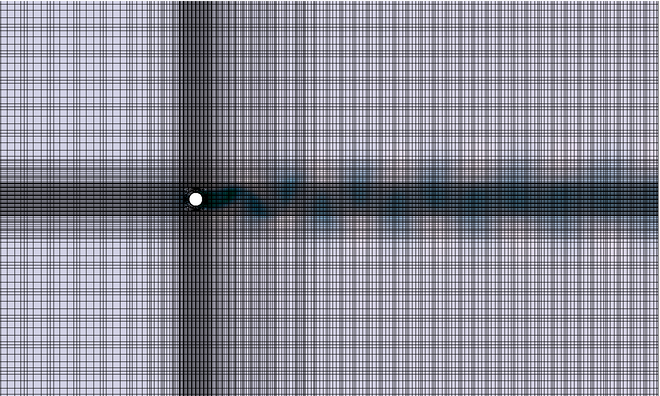
\includegraphics[width=0.39\textwidth]{i/nek.png}
\eframe
\end{document}
